\section{Data management considerations for AM}
\label{sec:DMC}

\subsection{AM design space considerations}
\label{subsec:DMC_design_space}
When attempting to optimize an AM workflow for a particular property, it is important to consider the size and complexity of the design space.
For a typical build plate, it's possible to consider 10+ variables solely based on printing parameters.
Depending on the resolution to which each parameter should be varied, the design space will likely be too large to experimentally determine each value.
Table\ref{table:design_space}, illustrates potential parameters to consider for a typical AM design space.
While it is common to explore varying 2-3 of these parameters at a time, to fully explore this space would necessitate 10$^9$ experiments!
The size of this parameter space indicates the value of data-driven exploration.
While it may be most valuable to seed the design exploration by performing orthogonal experiments first(which could be determined using dimensionality reduction techniques), typical experimental conditions facilitate fine exploration of a small subset of the design space.
For example, a build plate of 44 samples is likely to be all of the same composition with each sample only differing by their part orientation on the build plate.
This hindrance suggests that seeding your design space from the currently available or past experiments will lead to desired output more quickly.

\begin{table*}
    \renewcommand{\arraystretch}{0.8}
    \setlength{\tabcolsep}{5pt}
    \begin{center}
        \begin{tabular}{@{}llll@{}}
            \toprule
            \hline
             Parameter & range & step size & levels \\ \midrule
            \hline
            \hline
            Skin/Contour/Core laser parameters: & & & \\
            Power & 100-200 W & 10 W & 10 \\
            Scan speed & 500-1000 mm/s & 100 mm/s & 5 \\
            Spot size & 50-100 $\mu$m & 10 $\mu$m & 5 \\
            Energy density & 1-5 J/mm$^2$ & 1 J/mm$^2$ & 5 \\
            \hline
            Build parameters: & & & \\
            Polar angle & 0-90$^\circ$ & 30$^\circ$  & 4 \\
            Azimuth angle & 0-180$^\circ$ & 90$^\circ$  & 3 \\
            Sieve count & 0-10 & 2 & 5 \\
            Amount of recycled powder & 0-100\% & 10\% & 10 \\
            \hline
            Other parameters: & & & \\
            Blade direction & 0-300 mm & 10 mm  & 30 \\
            Transverse direction & 0-300 mm & 10 mm  & 30 \\
            Hatch spacing & 0.1-0.50 mm & 0.1 nm  & 5 \\
            \hline
            \bottomrule
        \end{tabular}
        \caption{Typical AM design space set up for determining PSP relationships. Multiplying the factorial yields 10$^6$ possible experiments.}
        \label{table:design_space}
    \end{center}
\end{table*}

\subsection{AM data generation and formatting considerations}
\label{subsec:DMC_data}
Given the complexity and time associated with synthesizing and characterizing an AM build plate, each experimental data point generated is costly.
To ensure capture of all process conditions our recent AM workflows[REFERENCE?] have employed the PIF data format.
Aligned with the FAIR data principles\cite{Wilkinson2016}, the PIF data format is a hierarchical json-based schema designed specifically to store materials data from the part level to the atomic level.
The pif files generated from these recent workflows have been stored online on the Citrination platform (adapt.citrination.com), allowing for data to be shared and analyzed across the entire organization.
Table\ref{table:data_tools} describes common file types and tools associated with AM data and workflows.

\begin{table*}
    \renewcommand{\arraystretch}{0.8}
    \setlength{\tabcolsep}{5pt}
    \begin{center}
        \begin{tabular}{@{}llll@{}}
            \toprule
            Data source (instrument/software) & file type & processing tools & "ML-ready" output \\ \midrule
            \hline
            \hline
            X-Ray tomography (Zeiss Xradia Versa) & .tiff & image featurizer & vectorized image \\
            X-Ray tomography (TRACR) & .txt, .csv & Python (pypif, pandas, citriantion-client) & porosity statistics \\
            X-Ray diffraction (Panalytical empyrean) & .xy & Python (pypif, csv, pandas) & XRD features (\% desired phase) \\
            Optical microscopy (Keyence VHX-5000) & .tiff & image featurizer & vectorized image (grain size and distributions) \\
            Uniaxial tensile testing (MTS 370) & .xy & Python (Hough transform algorithm) & real-valued mechanical properties \\
            Composition (TOF-SIMS) & & Python (pymatgen, matminer, magpie) & composition feature vectors \\
            Semi-structured web page & .html & Python (requests, beautifulsoup) & csv-formatted records \\
            Semi-structured pdf (txt-based) & .pdf & tabula, AbbyyFineReader, Python (pdftotext) & csv-formatted records \\
            ML packages & & Python (sklearn, tensorflow, keras, OpenCV) & \\
            \hline
            \bottomrule
        \end{tabular}
        \caption{Common tools and packages for preparing data for ML applications}
        \label{table:data_tools}
    \end{center}
\end{table*}


\subsection{Preparing data for machine learning}

For materials synthesis applications, signal from machine learning models is often limited by the amount of data and the speed at which data can be collected.
Many standard algorithms are suitable to correlate high-dimensional inputs and outputs in the AM design space.
However, random forest algorithms are particularly well-suited for AM synthesis optimization as they work well with small datasets and can be used for classification or regression.

To prepare experimentally generated data for input to a machine learning model, python scripting and other automation tools are typically employed.
For AM synthesis optimization, data is generated at many disparate sources.
For example, after a build plate is printed, the porosity of each sample is determined through X-ray tomography while other mechanical properties are determined through tensile testing.
Data collected this way is typically resolved through a master record in which data from many instruments and synthesis steps is stored.
Also, storing these data in a human and machine-readable format allows for quick error checking and data maniuplation to be performed while still being accessible for machine learning.
Table XX highlights a variety of computational tools and Python packages and their relevance to AM synthesis optimization.



\subsection{Sequential learning workflow}

%\begin{figure}
%  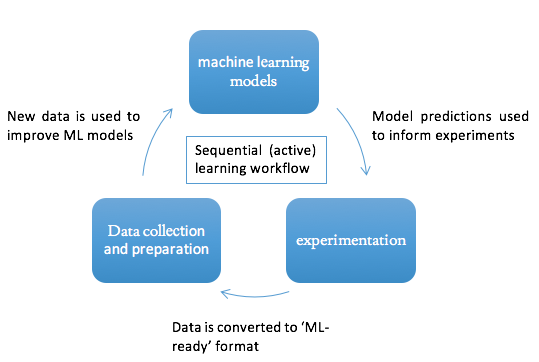
\includegraphics[width=0.75\linewidth]{Images/SL_workflow_placeholder.png}
%  \caption{Prelim idea for including a SL workflow figure.}
%  \label{fig:SL}
%\end{figure}


Often data necessary for quality models come from many disparate sources.

Raw data is often semi-structured (csv, html, txt) or un-structured (image, pdf, notebook)

To take data from semi- or non- structured formats, we employ traditional data digitization tools (digitizer.citrination.com, tabula)

Data needs to be stored in a machine-readable format and should adhere to FAIR principles [CITE].

Since we rarely work with 'big data' (datasets too large to be maintained in a local/non-distributed environment), txt based formats are ideal storage methods.

A PIF is a great example of an open-source and extensible data format that allows for data storage for atomic and macroscopic (part-level) data.

human-readable data formats = .txt, .json, PIF, lab notebook

machine-readiable data formats = .json, .txt, .pdf, .raw

Python is a robust, high-level language well-suited for use by the materials scientist.

Python allows for automation of data manipulation processes.

mats sci / ML focused python packages: sklearn, pypif, pymatgen, keras?, tensorflow
Data manipulation and visualization: numpy, scipy, matplotlib, beautifulsoup, requests, pypif
ML frameworks: sklearn, tensorflow, keras